\documentclass{standalone}
\usepackage{tikz}
\usepackage{amsmath}
\usetikzlibrary{shapes, arrows, chains}
\tikzstyle{line} = [draw, -latex']
\begin{document}

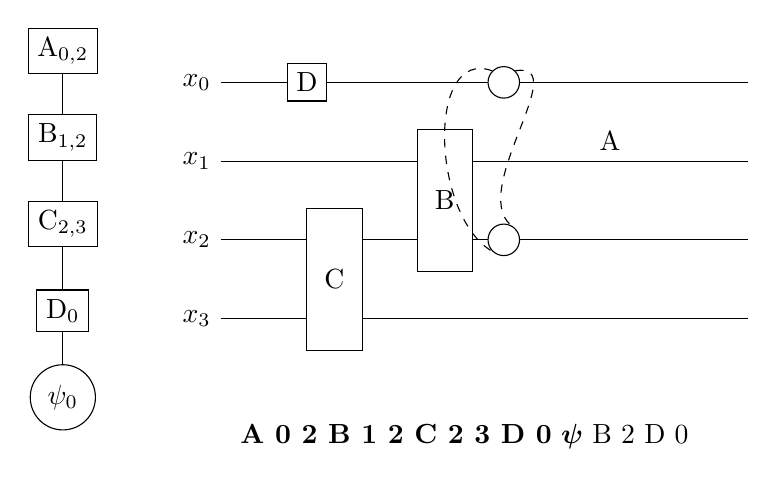
\begin{tikzpicture}
	\def\yl{-1}
	\def\xl{7}
	\def\mx{1.7}
	\def\my{4}
	\node (x0) at (\mx,\my) {$x_0$};
	\node (x1) at (\mx, \yl+\my) {$x_1$};
	\node (x2) at (\mx, 2*\yl+\my) {$x_2$};
	\node (x3) at (\mx, 3*\yl+\my) {$x_3$};
	\coordinate (l0) at (\xl+\mx, \my);
	\coordinate (l1) at (\xl+\mx, \yl+\my);
	\coordinate (l2) at (\xl+\mx, 2*\yl+\my);
	\coordinate (l3) at (\xl+\mx, 3*\yl+\my);
	\draw (x0) -- (l0);
	\draw (x1) -- (l1);
	\draw (x2) -- (l2);
	\draw (x3) -- (l3);
	\node[rectangle,draw=black,fill=white] at (0.2*\xl+\mx, \my) {D};
	\draw[fill=white] (0.4*\xl+\mx, 0.6*\yl+\my) -- (0.5*\xl+\mx, 0.6*\yl+\my) -- 
	(0.5*\xl+\mx, 2.4*\yl+\my) -- (0.4*\xl+\mx, 2.4*\yl+\my) -- cycle;
	\node at (0.45*\xl+\mx, 1.5*\yl+\my) {B};
	\draw[fill=white] (0.2*\xl+\mx, 1.6*\yl+\my) -- (0.3*\xl+\mx, 1.6*\yl+\my) -- 
	(0.3*\xl+\mx, 3.4*\yl+\my) -- (0.2*\xl+\mx, 3.4*\yl+\my) -- cycle;
	\node at (0.25*\xl+\mx, 2.5*\yl+\my) {C};
	\node[circle, draw=black, minimum size=0.4cm, fill=white] (A0) at (0.8*\xl, \my) {};
	\node[circle, draw=black, minimum size=0.4cm, fill=white] (A1) at (0.8*\xl, 2*\yl+\my) {};
	\draw[dashed] (A0.north west) to[out=160, in=150] (A1.south west);
	\draw[dashed] (A0.north east) to[out=10, in=150] (A1.north east);
	\node at (0.75*\xl+\mx, 0.75*\yl+\my) {A};
%%%%
	\def\yn{1.1}
	\def\xn{2.5}
	\node[circle, draw=black] (x0) at (0, 0) {$\psi_0$};
	\node[rectangle,draw=black,fill=white] (D) at (0, \yn) {D$_0$};
	\node[rectangle,draw=black,fill=white] (C) at (0, 2*\yn) {C$_{2,3}$};
	\node[rectangle,draw=black,fill=white] (B) at (0, 3*\yn) {B$_{1,2}$};
	\node[rectangle,draw=black,fill=white] (A) at (0, 4*\yn) {A$_{0,2}$};
	\draw (x0) -- (D);	
	\draw (D) -- (C);
	\draw (C) -- (B);
	\draw (B) -- (A);
%%%%
	\node at (3*\mx, -0.5) {\textbf{A 0 2 B 1 2 C 2 3 D 0} $\boldsymbol{\psi}$ B 2 D 0};	
\end{tikzpicture}
\end{document}

